\documentclass[11pt,a4paper]{article}

\usepackage[
    a4paper,
    left=15mm,
    right=15mm,
    top=30mm,
    bottom=25mm,
    headheight=25mm
]{geometry}
\usepackage{graphicx}
\usepackage{polski}
\usepackage[utf8]{inputenc}
\usepackage{enumerate}
\usepackage{comment}
\usepackage{fancyhdr}
\usepackage{hyperref}
\usepackage{indentfirst}
\usepackage{multirow}
\usepackage{multicol}
\usepackage{float}
\usepackage{amsmath}
\usepackage{amssymb}
\usepackage{wrapfig}
\usepackage{layout}
\usepackage{textcomp}
\usepackage[center]{caption}
\usepackage{subcaption}
\usepackage{siunitx}
\usepackage[mathscr]{euscript}
\usepackage{xcolor,colortbl}
\usepackage{setspace}
\usepackage{algorithm}
\usepackage[rightComments=false]{algpseudocodex}
\usepackage{listings}
\usepackage{amsthm}
\usepackage{needspace}

% no lone first/last lines of a paragraph on a page
\widowpenalty=10000
\clubpenalty=10000
\displaywidowpenalty=10000

\sisetup{output-exponent-marker=\ensuremath{\mathrm{e}}, output-decimal-marker={,}}
\algrenewcommand\algorithmicprocedure{\textbf{Procedura}}
\algrenewcommand\algorithmicfor{\textbf{Dla}}
\algrenewcommand\algorithmicdo{\textbf{powtarzaj}}
\algrenewcommand\algorithmicwhile{\textbf{Dopóki}}
\algrenewcommand\algorithmicloop{\textbf{Powtarzaj}}
\algrenewcommand\algorithmicif{\textbf{Jeżeli}}
\algrenewcommand\algorithmicelse{\textbf{Inaczej}}
\algrenewcommand\algorithmicthen{\textbf{wykonaj}}
\algrenewcommand\algorithmicend{\textbf{Koniec}}
\algrenewcommand\algorithmicreturn{\textbf{zwróć}}

\newenvironment{algorytm}[1][htb]
  {\par\bigskip\floatname{algorithm}{}\renewcommand{\thealgorithm}{}
   \begin{algorithm}[#1]%
  }{\end{algorithm}\par\bigskip}

\renewcommand{\baselinestretch}{1.18}
\renewcommand\thesubfigure{\roman{subfigure}}

\renewcommand\lstlistingname{Kod}
\lstset{
    language=Java,
    basicstyle=\ttfamily\footnotesize,
    keywordstyle=\bfseries,
    commentstyle=\itshape\color{gray},
    numbers=left,
    numberstyle=\tiny\color{gray},
    numbersep=8pt,
    frame=tb,
    xleftmargin=6mm,
    columns=fullflexible,
    keepspaces=true,
    showstringspaces=false,
    tabsize=4,
    captionpos=b,
    breaklines=true,
    postbreak=\mbox{\textcolor{gray}{$\hookrightarrow$}\space}
}

\pagestyle{fancy}
\fancyhead[L]{
    
\includegraphics[height=12mm]{img/agh-logo.jpg}
}
\fancyhead[R]{}

\author{Szymon Iwaniuk}
\title{
    
\includegraphics[height=45mm]{img/agh-logo.jpg}
    \vspace{10mm}
    \\
    Producenci i konsumenci z losową wielkością porcji}
\date{Teoria Współbieżności 2025/2026, laboratorium 4 \\ 30 października 2026}

\begin{document}

\maketitle
\tableofcontents
\pagebreak

\section{Wstęp}
\subsection{Treść zadania}
\textbf{Producenci i konsumenci z losową ilością pobieranych i wstawianych porcji}
\begin{itemize}
    \item Bufor o rozmiarze $2M$
    \item Jest $m$ producentów i $n$ konsumentów
    \item Producent wstawia do bufora losową liczbę elementów (nie więcej niż $M$)
    \item Konsument pobiera losową liczbę elementów (nie więcej niż $M$)
    \item Zaimplementować przy pomocy monitorów Javy oraz mechanizmów Java Concurrency Utilities
    \item Przeprowadzić porównanie wydajności (np. czas wykonywania) vs. różne parametry,
          zrobić wykresy i je skomentować
\end{itemize}

\subsection{Opis rozwiązania}
Porównujemy cztery implementacje bufora:
\begin{itemize}
    \item \textbf{monitor} -- metody \texttt{synchronized} z \texttt{wait()} i \texttt{notifyAll()},
    \item \textbf{ReentrantLock, 2 warunki} -- osobne warunki \texttt{notFull} i \texttt{notEmpty},
    \item \textbf{ReentrantLock, 4 warunki} -- na miejsce w buforze czeka tylko pierwszy
          producent (konsument), a pozostali czekają za nim,
    \item \textbf{4 warunki + kolejka biletowa} -- jak wyżej, ale kolejność wątków
          wyznacza numer pobrany przy wejściu.
\end{itemize}
Dwie pierwsze implementacje są rozwiązaniami ,,naiwnymi'': wątek, który chce dużej porcji,
może być wielokrotnie wyprzedzany przez wątki chcące małych porcji.
Rozwiązanie z czterema warunkami usuwa ten problem dla wielkości porcji,
ale pomiary pokazały, że w Javie nie zapewnia kolejności między wątkami
(rozdział \ref{sec:barging}). Dlatego dodaliśmy czwartą implementację z kolejką biletową
i sprawdzamy, ile kosztuje pełna sprawiedliwość.

Razem ze sprawozdaniem zawarty jest kod w języku \texttt{Java} zawierający
wszystkie implementacje, program wykonujący pomiary
oraz skrypt służący do generowania zawartych w dokumencie wykresów.

\section{Specyfikacja narzędzi i sprzętu}
Program został napisany w języku \texttt{Java 27} i uruchomiony na maszynie wirtualnej
\texttt{OpenJDK}, na komputerze z procesorem \texttt{Apple M4} (architektura \texttt{ARM64},
10 rdzeni: 4 wydajnościowe i 6 energooszczędnych), \texttt{16 GB} zunifikowanej pamięci
\texttt{LPDDR5} i systemem operacyjnym \texttt{macOS 26}.
Do wygenerowania wykresów użyty został \texttt{Python} z biblioteką \texttt{matplotlib}.

\subsection{Metoda pomiaru}
Żeby każdy przebieg miał koniec, przez bufor przesyłamy ustaloną liczbę elementów
$T = 20\,000 \cdot \frac{M + 1}{2}$. Średnia porcja ma $\frac{M+1}{2}$ elementów,
więc producenci wykonują łącznie około $20\,000$ wstawień niezależnie od $M$.
Wątek losuje porcję, a bufor przycina ją do liczby elementów, które zostały do wstawienia
(pobrania). Gdy nic nie zostało, \texttt{put} i \texttt{take} zwracają \texttt{false} i wątek kończy pracę.
W pętlach wątków nie ma \texttt{Thread.sleep}, więc mierzymy koszt synchronizacji, a nie czas uśpienia.

Wszystkie wątki startują jednocześnie po zwolnieniu zatrzasku \texttt{CountDownLatch}.
Czas mierzymy zegarem \texttt{System.nanoTime()} od startu do zakończenia ostatniego wątku
(\texttt{join}). Przed pomiarami wykonujemy kilka przebiegów rozgrzewających kompilator JIT.
Każdą konfigurację uruchamiamy trzy razy i bierzemy medianę.
Dodatkowo każdy wątek mierzy czas każdego wywołania \texttt{put} i \texttt{take},
grupując wyniki według wielkości porcji w 10 przedziałach, i liczy swoje wywołania.
Równomierność podziału pracy między wątki mierzymy indeksem Jaina
\[
    J(x_1, \dots, x_k) = \frac{\left(\sum_{i=1}^{k} x_i\right)^2}{k \sum_{i=1}^{k} x_i^2},
\]
gdzie $x_i$ to liczba udanych wywołań $i$-tego producenta (konsumenta).
$J = 1$, gdy wszystkie wątki wykonały tyle samo operacji, a $J = \frac{1}{k}$,
gdy całą pracę wykonał jeden wątek. Na wykresach podajemy mniejszy z indeksów
producentów i konsumentów.

Parametry: $M \in \{100, 1000, 10\,000\}$, $m, n \in \{1, 2, 4, 8, 16, 32\}$.
Po każdym przebiegu sprawdzamy, że bufor jest pusty i przesłano dokładnie $T$ elementów.

\section{Algorytmy}
W pseudokodzie $s$ oznacza liczbę elementów w buforze, $2M - s$ liczbę wolnych miejsc,
a $r_p$ i $r_k$ liczbę elementów, które zostały do wstawienia i do pobrania.
Procedura \textsc{take} jest symetryczna do \textsc{put}: zamienia rolami $s$ i $2M - s$,
$r_p$ i $r_k$ oraz warunki producentów i konsumentów, dlatego jej nie powtarzamy.

\needspace{12\baselineskip}
\subsection{Rozwiązanie naiwne}
\label{sec:naive}
Obie naiwne implementacje działają tak samo. Monitor ma jeden zbiór oczekujących,
więc \texttt{notifyAll()} budzi wszystkie wątki. Wersja z \texttt{ReentrantLock}
budzi tylko wątki drugiej strony, a własną stronę budzi jedynie po wyczerpaniu $r_p$,
żeby pozostali producenci mogli się zakończyć.

\begin{algorytm}[H]
\setstretch{1.4}
\begin{algorithmic}[1]
    \Procedure{put}{$k$}
        \Loop
            \If{$r_p = 0$}
                \State \Return \texttt{false}
            \EndIf
            \State $k' \gets \min(k, r_p)$
            \If{$2M - s \ge k'$}
                \State wstaw $k'$ elementów, $r_p \gets r_p - k'$
                \State \textsc{signalAll}(\textit{notEmpty}) \Comment{monitor: \textsc{notifyAll}}
                \State \Return \texttt{true}
            \EndIf
            \State \textsc{await}(\textit{notFull}) \Comment{monitor: \textsc{wait}}
        \EndLoop
    \EndProcedure
\end{algorithmic}
\caption{Wstawianie w rozwiązaniu naiwnym}
\end{algorytm}

Producent chcący $M$ elementów potrzebuje połowy bufora. Po każdym pobraniu budzą się
wszyscy producenci, a pierwszy z nich, który dostanie blokadę, zajmuje zwolnione miejsce.
Producenci z małymi porcjami mieszczą się częściej, więc producent z dużą porcją
może czekać bardzo długo (zagłodzenie).

\needspace{14\baselineskip}
\subsection{Rozwiązanie z czterema warunkami}
Wątki jednej strony ustawiają się w kolejce na warunku \textit{otherProducers}.
Tylko pierwszy producent czeka na wolne miejsce na warunku \textit{firstProducer},
więc nikt nie zajmie miejsca, na które on czeka. Po wyjściu oddaje miejsce
następnemu w kolejce (wiersz 14).

\begin{algorytm}[H]
\setstretch{1.4}
\begin{algorithmic}[1]
    \Procedure{put}{$k$}
        \While{\textit{producerFirst}}
            \State \textsc{await}(\textit{otherProducers})
        \EndWhile
        \State $\textit{producerFirst} \gets \texttt{true}$
        \Loop
            \If{$r_p = 0$}
                \State \textbf{wyjdź z pętli} z wynikiem \texttt{false}
            \EndIf
            \State $k' \gets \min(k, r_p)$
            \If{$2M - s \ge k'$}
                \State wstaw $k'$ elementów, $r_p \gets r_p - k'$
                \State \textsc{signal}(\textit{firstConsumer})
                \State \textbf{wyjdź z pętli} z wynikiem \texttt{true}
            \EndIf
            \State \textsc{await}(\textit{firstProducer})
        \EndLoop
        \State $\textit{producerFirst} \gets \texttt{false}$, \ \textsc{signal}(\textit{otherProducers})
        \State \Return wynik
    \EndProcedure
\end{algorithmic}
\caption{Wstawianie w rozwiązaniu z czterema warunkami}
\end{algorytm}

Konsument po pobraniu budzi \textit{firstProducer}, czyli dokładnie jednego producenta.
Gdy $r_p$ spadnie do zera, każdy kolejny producent wychodzi od razu i budzi następnego,
więc wszystkie wątki kończą pracę.

\needspace{10\baselineskip}
\subsection{Wyprzedzanie przy zwolnieniu blokady}
\label{sec:barging}
Domyślny \texttt{ReentrantLock} nie jest sprawiedliwy: wątek obudzony przez \textsc{signal}
musi jeszcze ponownie zdobyć blokadę, a w tym czasie może ją przejąć dowolny inny wątek.
Producent, który właśnie wyszedł z \textsc{put} w wierszu 14, od razu wywołuje \textsc{put}
ponownie, widzi $\textit{producerFirst} = \texttt{false}$ i znów zostaje pierwszy,
zanim obudzony wątek dostanie procesor. W naszym pomiarze dla $M = 1000$
i 16 producentów jeden wątek wykonał wszystkie $20\,028$ wstawień, a pozostałe 15 żadnego.
Rozwiązanie jest więc sprawiedliwe względem wielkości porcji, ale głodzi wątki.

Kolejka biletowa usuwa ten problem. Każdy wątek przy wejściu pobiera kolejny numer
i zostaje pierwszy dopiero wtedy, gdy obsługiwany jest jego numer. Kolejność obsługi
jest więc kolejnością wejścia i nikt nie może się wepchnąć.

\begin{algorytm}[H]
\setstretch{1.4}
\begin{algorithmic}[1]
    \Procedure{put}{$k$}
        \State $b \gets \textit{ticket}$, \ $\textit{ticket} \gets \textit{ticket} + 1$
        \While{$b \ne \textit{served}$}
            \State \textsc{await}(\textit{otherProducers})
        \EndWhile
        \State \textit{wynik} $\gets$ wiersze 5--13 rozwiązania z czterema warunkami
        \State $\textit{served} \gets \textit{served} + 1$, \ \textsc{signalAll}(\textit{otherProducers})
        \State \Return wynik
    \EndProcedure
\end{algorithmic}
\caption{Wstawianie z kolejką biletową}
\end{algorytm}

\textsc{signal} budzi dowolny czekający wątek, a nie koniecznie właściciela następnego numeru,
dlatego w wierszu 6 budzimy wszystkich, a dalej przechodzi tylko jeden.

\pagebreak
\section{Implementacja}
Poniżej znajduje się pełny kod programu. Każda klasa jest w osobnym pliku w katalogu \texttt{src}.

Klasa \textbf{Buffer} jest wspólną bazą wszystkich implementacji. Przechowuje elementy w buforze cyklicznym o rozmiarze $2M$ i liczniki elementów, które zostały do wstawienia i pobrania. Metoda \texttt{create} wybiera implementację po nazwie.

\begin{lstlisting}[caption={Klasa \textbf{Buffer} (\texttt{src/Buffer.java})}]
/**
 * Bounded buffer of capacity 2M with a fixed number of elements to pass through it.
 * put/take move min(want, remaining) elements and return false once nothing is left,
 * so every producer and consumer ends without being interrupted.
 */
abstract class Buffer {
    private final int[] data;
    private int head = 0;
    protected int size = 0;
    protected long toProduce;
    protected long toConsume;

    Buffer(int capacity, long total) {
        data = new int[capacity];
        toProduce = total;
        toConsume = total;
    }

    abstract boolean put(int want) throws InterruptedException;

    abstract boolean take(int want) throws InterruptedException;

    protected int free() {
        return data.length - size;
    }

    protected void insert(int n) {
        for (int i = 0; i < n; i++) {
            data[(head + size) % data.length] = 1;
            size++;
        }
        toProduce -= n;
    }

    protected void remove(int n) {
        for (int i = 0; i < n; i++) {
            data[head] = 0;
            head = (head + 1) % data.length;
            size--;
        }
        toConsume -= n;
    }

    static Buffer create(String impl, int capacity, long total) {
        return switch (impl) {
            case "monitor" -> new MonitorBuffer(capacity, total);
            case "lock" -> new LockBuffer(capacity, total);
            case "fair" -> new FairBuffer(capacity, total);
            case "ticket" -> new TicketBuffer(capacity, total);
            default -> throw new IllegalArgumentException(impl);
        };
    }
}
\end{lstlisting}

Klasa \textbf{MonitorBuffer} to rozwiązanie naiwne na monitorze Javy. Cała metoda jest sekcją krytyczną, a \texttt{wait()} zwalnia monitor na czas oczekiwania.

\begin{lstlisting}[caption={Klasa \textbf{MonitorBuffer} (\texttt{src/MonitorBuffer.java})}]
/** Java monitor: synchronized methods, wait() and notifyAll() on a single wait set. */
class MonitorBuffer extends Buffer {
    MonitorBuffer(int capacity, long total) {
        super(capacity, total);
    }

    @Override
    synchronized boolean put(int want) throws InterruptedException {
        while (true) {
            if (toProduce == 0) return false;
            int n = (int) Math.min(want, toProduce);
            if (free() >= n) {
                insert(n);
                notifyAll();
                return true;
            }
            wait();
        }
    }

    @Override
    synchronized boolean take(int want) throws InterruptedException {
        while (true) {
            if (toConsume == 0) return false;
            int n = (int) Math.min(want, toConsume);
            if (size >= n) {
                remove(n);
                notifyAll();
                return true;
            }
            wait();
        }
    }
}
\end{lstlisting}

Klasa \textbf{LockBuffer} to rozwiązanie naiwne z \texttt{ReentrantLock} i dwoma warunkami: producenci czekają na \texttt{notFull}, a konsumenci na \texttt{notEmpty}.

\begin{lstlisting}[caption={Klasa \textbf{LockBuffer} (\texttt{src/LockBuffer.java})}]
import java.util.concurrent.locks.Condition;
import java.util.concurrent.locks.ReentrantLock;

/** Java Concurrency Utilities: ReentrantLock with separate conditions for producers and consumers. */
class LockBuffer extends Buffer {
    private final ReentrantLock lock = new ReentrantLock();
    private final Condition notFull = lock.newCondition();
    private final Condition notEmpty = lock.newCondition();

    LockBuffer(int capacity, long total) {
        super(capacity, total);
    }

    @Override
    boolean put(int want) throws InterruptedException {
        lock.lock();
        try {
            while (true) {
                if (toProduce == 0) return false;
                int n = (int) Math.min(want, toProduce);
                if (free() >= n) {
                    insert(n);
                    notEmpty.signalAll();
                    if (toProduce == 0) notFull.signalAll(); // let the other producers finish
                    return true;
                }
                notFull.await();
            }
        } finally {
            lock.unlock();
        }
    }

    @Override
    boolean take(int want) throws InterruptedException {
        lock.lock();
        try {
            while (true) {
                if (toConsume == 0) return false;
                int n = (int) Math.min(want, toConsume);
                if (size >= n) {
                    remove(n);
                    notFull.signalAll();
                    if (toConsume == 0) notEmpty.signalAll(); // let the other consumers finish
                    return true;
                }
                notEmpty.await();
            }
        } finally {
            lock.unlock();
        }
    }
}
\end{lstlisting}

Klasa \textbf{FairBuffer} to rozwiązanie z czterema warunkami. Blok \texttt{finally} zwalnia miejsce pierwszego producenta (konsumenta) niezależnie od tego, którą drogą metoda się kończy.

\begin{lstlisting}[caption={Klasa \textbf{FairBuffer} (\texttt{src/FairBuffer.java})}]
import java.util.concurrent.locks.Condition;
import java.util.concurrent.locks.ReentrantLock;

/**
 * Four conditions: only the first producer (consumer) in line waits for space (elements),
 * the rest queue behind it, so a large portion cannot be overtaken by smaller ones.
 */
class FairBuffer extends Buffer {
    private final ReentrantLock lock = new ReentrantLock();
    private final Condition firstProducer = lock.newCondition();
    private final Condition otherProducers = lock.newCondition();
    private final Condition firstConsumer = lock.newCondition();
    private final Condition otherConsumers = lock.newCondition();
    private boolean producerFirst = false;
    private boolean consumerFirst = false;

    FairBuffer(int capacity, long total) {
        super(capacity, total);
    }

    @Override
    boolean put(int want) throws InterruptedException {
        lock.lock();
        try {
            while (producerFirst) otherProducers.await();
            producerFirst = true;
            try {
                while (true) {
                    if (toProduce == 0) return false;
                    int n = (int) Math.min(want, toProduce);
                    if (free() >= n) {
                        insert(n);
                        firstConsumer.signal();
                        return true;
                    }
                    firstProducer.await();
                }
            } finally {
                producerFirst = false;
                otherProducers.signal();
            }
        } finally {
            lock.unlock();
        }
    }

    @Override
    boolean take(int want) throws InterruptedException {
        lock.lock();
        try {
            while (consumerFirst) otherConsumers.await();
            consumerFirst = true;
            try {
                while (true) {
                    if (toConsume == 0) return false;
                    int n = (int) Math.min(want, toConsume);
                    if (size >= n) {
                        remove(n);
                        firstProducer.signal();
                        return true;
                    }
                    firstConsumer.await();
                }
            } finally {
                consumerFirst = false;
                otherConsumers.signal();
            }
        } finally {
            lock.unlock();
        }
    }
}
\end{lstlisting}

Klasa \textbf{TicketBuffer} różni się od \textbf{FairBuffer} tylko wejściem i wyjściem: wątek czeka na swój numer, a przy wyjściu obsługiwany jest następny numer.

\begin{lstlisting}[caption={Klasa \textbf{TicketBuffer} (\texttt{src/TicketBuffer.java})}]
import java.util.concurrent.locks.Condition;
import java.util.concurrent.locks.ReentrantLock;

/**
 * FairBuffer with a ticket queue: each thread takes a number and becomes first only when
 * its number is served, so a thread that grabs the lock right after leaving cannot jump
 * ahead of the threads already waiting.
 */
class TicketBuffer extends Buffer {
    private final ReentrantLock lock = new ReentrantLock();
    private final Condition firstProducer = lock.newCondition();
    private final Condition otherProducers = lock.newCondition();
    private final Condition firstConsumer = lock.newCondition();
    private final Condition otherConsumers = lock.newCondition();
    private long producerTicket = 0, producerServed = 0;
    private long consumerTicket = 0, consumerServed = 0;

    TicketBuffer(int capacity, long total) {
        super(capacity, total);
    }

    @Override
    boolean put(int want) throws InterruptedException {
        lock.lock();
        try {
            long ticket = producerTicket++;
            while (ticket != producerServed) otherProducers.await();
            try {
                while (true) {
                    if (toProduce == 0) return false;
                    int n = (int) Math.min(want, toProduce);
                    if (free() >= n) {
                        insert(n);
                        firstConsumer.signal();
                        return true;
                    }
                    firstProducer.await();
                }
            } finally {
                producerServed++;
                otherProducers.signalAll(); // only the owner of the next ticket proceeds
            }
        } finally {
            lock.unlock();
        }
    }

    @Override
    boolean take(int want) throws InterruptedException {
        lock.lock();
        try {
            long ticket = consumerTicket++;
            while (ticket != consumerServed) otherConsumers.await();
            try {
                while (true) {
                    if (toConsume == 0) return false;
                    int n = (int) Math.min(want, toConsume);
                    if (size >= n) {
                        remove(n);
                        firstProducer.signal();
                        return true;
                    }
                    firstConsumer.await();
                }
            } finally {
                consumerServed++;
                otherConsumers.signalAll();
            }
        } finally {
            lock.unlock();
        }
    }
}
\end{lstlisting}

Klasa \textbf{Main} tworzy wątki producentów i konsumentów dla wszystkich konfiguracji, mierzy czas, liczy indeks Jaina i zapisuje wyniki do plików CSV, z których skrypt w Pythonie rysuje wykresy.

\begin{lstlisting}[caption={Klasa \textbf{Main} (\texttt{src/Main.java})}]
import java.io.FileWriter;
import java.io.IOException;
import java.io.PrintWriter;
import java.util.ArrayList;
import java.util.Arrays;
import java.util.List;
import java.util.SplittableRandom;
import java.util.concurrent.CountDownLatch;

/**
 * Runs every implementation for a grid of M, producer and consumer counts and writes
 * csv/times.csv (wall time) and csv/waits.csv (time spent in put/take per portion size).
 */
public class Main {
    static final String[] IMPLS = {"monitor", "lock", "fair", "ticket"};
    static final int[] PORTIONS = {100, 1000, 10000};
    static final int[] THREADS = {1, 2, 4, 8, 16, 32};
    static final int OPS = 20_000;   // expected number of put calls in one run
    static final int REPS = 3;
    static final int BUCKETS = 10;   // portion sizes 1..M split into equal ranges

    /** Wait time histogram of one thread, merged after the run. */
    static final class Stats {
        final long[] count = new long[BUCKETS];
        final long[] sumNs = new long[BUCKETS];
        final long[] maxNs = new long[BUCKETS];

        void record(int bucket, long ns) {
            count[bucket]++;
            sumNs[bucket] += ns;
            maxNs[bucket] = Math.max(maxNs[bucket], ns);
        }

        void merge(Stats o) {
            for (int b = 0; b < BUCKETS; b++) {
                count[b] += o.count[b];
                sumNs[b] += o.sumNs[b];
                maxNs[b] = Math.max(maxNs[b], o.maxNs[b]);
            }
        }
    }

    /** Jain's index of calls per thread: 1 when all threads did the same work, 1/k when one did all. */
    static double jain(Stats[] stats, int from, int to) {
        double sum = 0, sumSq = 0;
        for (int t = from; t < to; t++) {
            long calls = Arrays.stream(stats[t].count).sum();
            sum += calls;
            sumSq += (double) calls * calls;
        }
        return sumSq == 0 ? 1 : sum * sum / ((to - from) * sumSq);
    }

    record Result(long timeNs, Stats producers, Stats consumers, double jainProducers, double jainConsumers) {}

    static Result run(String impl, int m, int producers, int consumers, long seed) throws InterruptedException {
        long total = (long) OPS * (m + 1) / 2;
        Buffer buffer = Buffer.create(impl, 2 * m, total);
        CountDownLatch ready = new CountDownLatch(producers + consumers);
        CountDownLatch start = new CountDownLatch(1);
        List<Thread> threads = new ArrayList<>();
        Stats[] stats = new Stats[producers + consumers];

        for (int t = 0; t < producers + consumers; t++) {
            boolean producer = t < producers;
            Stats s = stats[t] = new Stats();
            SplittableRandom rnd = new SplittableRandom(seed * 1_000 + t);
            threads.add(new Thread(() -> {
                try {
                    ready.countDown();
                    start.await();
                    while (true) {
                        int want = rnd.nextInt(m) + 1;
                        long t0 = System.nanoTime();
                        boolean ok = producer ? buffer.put(want) : buffer.take(want);
                        if (!ok) break;
                        s.record((want - 1) * BUCKETS / m, System.nanoTime() - t0);
                    }
                } catch (InterruptedException e) {
                    Thread.currentThread().interrupt();
                }
            }));
        }
        for (Thread th : threads) th.start();
        ready.await();
        long t0 = System.nanoTime();
        start.countDown();
        for (Thread th : threads) th.join();
        long elapsed = System.nanoTime() - t0;

        if (buffer.size != 0 || buffer.toProduce != 0 || buffer.toConsume != 0)
            throw new IllegalStateException(impl + ": buffer not drained");
        Stats p = new Stats(), c = new Stats();
        for (int t = 0; t < stats.length; t++) (t < producers ? p : c).merge(stats[t]);
        return new Result(elapsed, p, c, jain(stats, 0, producers), jain(stats, producers, stats.length));
    }

    static void writeWaits(PrintWriter w, String impl, int m, int producers, int consumers, String role, Stats s) {
        for (int b = 0; b < BUCKETS; b++) {
            if (s.count[b] == 0) continue;
            w.printf("%s,%d,%d,%d,%s,%d,%d,%d,%.3f,%.3f%n", impl, m, producers, consumers, role,
                    b * m / BUCKETS + 1, (b + 1) * m / BUCKETS, s.count[b],
                    s.sumNs[b] / 1e3 / s.count[b], s.maxNs[b] / 1e3);
        }
    }

    public static void main(String[] args) throws IOException, InterruptedException {
        String out = args.length > 0 ? args[0] : "csv";

        // JIT warm-up, results discarded
        for (String impl : IMPLS)
            for (int i = 0; i < 5; i++) run(impl, 1000, 4, 4, i);

        try (PrintWriter times = new PrintWriter(new FileWriter(out + "/times.csv"));
             PrintWriter waits = new PrintWriter(new FileWriter(out + "/waits.csv"))) {
            times.println("impl,M,producers,consumers,rep,time_ms,jain_producers,jain_consumers");
            waits.println("impl,M,producers,consumers,role,portion_lo,portion_hi,count,mean_us,max_us");
            for (int m : PORTIONS)
                for (int p : THREADS)
                    for (int c : THREADS) {
                        for (String impl : IMPLS) {
                            Stats ps = new Stats(), cs = new Stats();
                            double[] ms = new double[REPS];
                            for (int r = 0; r < REPS; r++) {
                                Result res = run(impl, m, p, c, r);
                                ms[r] = res.timeNs() / 1e6;
                                times.printf("%s,%d,%d,%d,%d,%.3f,%.4f,%.4f%n", impl, m, p, c, r, ms[r], res.jainProducers(), res.jainConsumers());
                                ps.merge(res.producers());
                                cs.merge(res.consumers());
                            }
                            writeWaits(waits, impl, m, p, c, "producer", ps);
                            writeWaits(waits, impl, m, p, c, "consumer", cs);
                            Arrays.sort(ms);
                            System.out.printf("M=%-5d p=%-2d c=%-2d %-7s median %8.1f ms%n", m, p, c, impl, ms[REPS / 2]);
                        }
                        times.flush();
                    }
        }
    }
}
\end{lstlisting}

\pagebreak
\section{Wyniki}
\subsection{Czas wykonania a liczba wątków}
\textbf{Rysunek 1} pokazuje czas przesłania wszystkich elementów, gdy producentów i konsumentów
jest tyle samo. Oś czasu jest logarytmiczna, bo kolejka biletowa jest wolniejsza o rząd wielkości.

\begin{figure}[H]
    \centering
    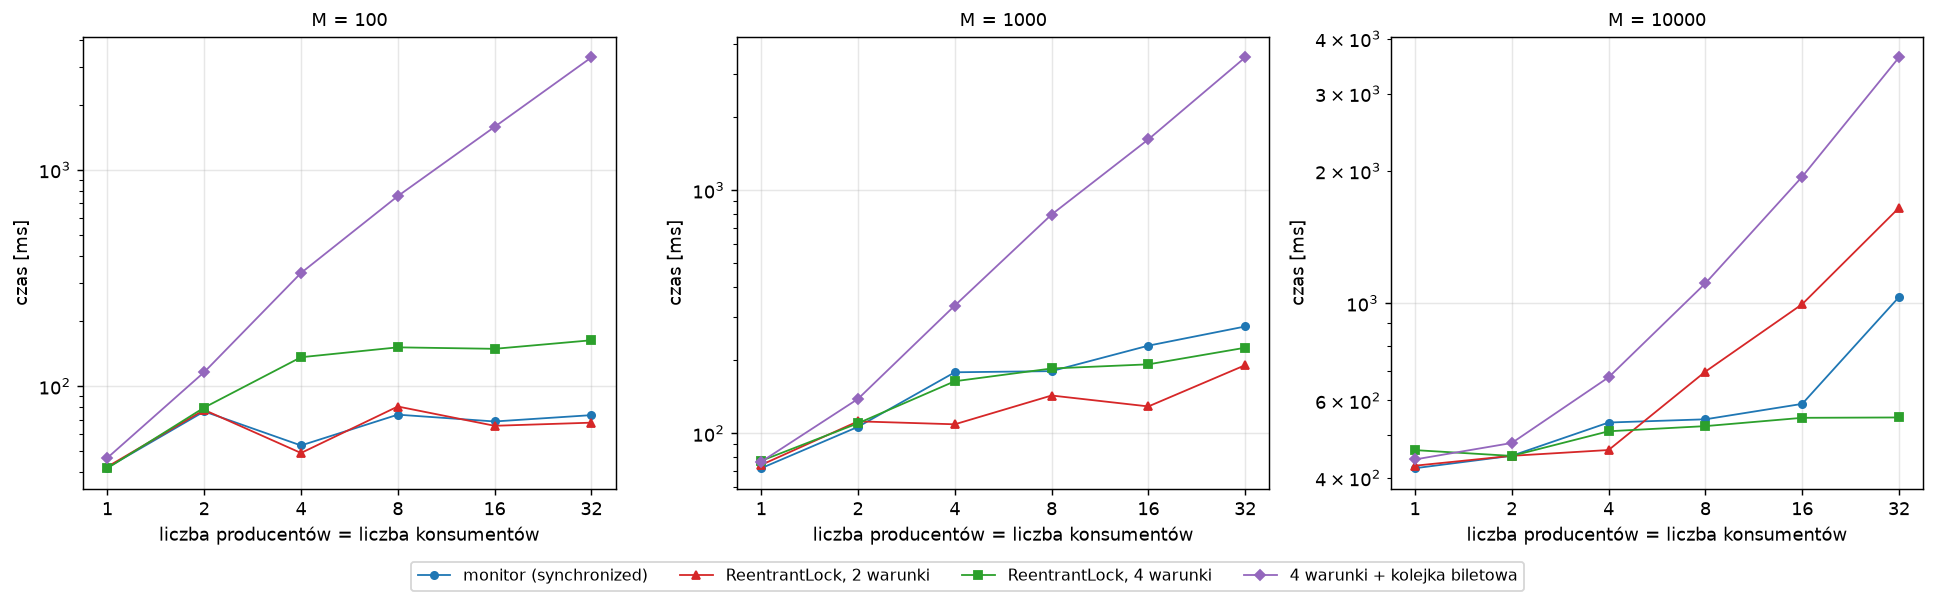
\includegraphics[width=\textwidth]{img/time_threads.png}
    \caption{Czas wykonania w zależności od liczby wątków dla $m = n$}
\end{figure}

Dla jednego producenta i jednego konsumenta wszystkie implementacje mają ten sam czas,
bo nie ma rywalizacji o blokadę. Czas rośnie z $M$ (42 ms dla $M = 100$, 420 ms dla $M = 10\,000$),
bo przy stałej liczbie wywołań każde wywołanie kopiuje średnio $\frac{M+1}{2}$ elementów.

Rozwiązania naiwne zwalniają umiarkowanie dla małych porcji, ale dla $M = 10\,000$
i 32 parach wątków są 2--4 razy wolniejsze niż dla jednej pary.
Po każdej operacji \texttt{notifyAll()} lub \texttt{signalAll()} budzi wszystkie wątki
drugiej strony, choć zwykle tylko jeden z nich może cokolwiek zrobić.
Rozwiązanie z czterema warunkami budzi dokładnie jeden wątek i jego czas prawie nie zależy
od liczby wątków. Kolejka biletowa jest najwolniejsza, a jej czas rośnie liniowo z liczbą wątków.

\textbf{Tabela 1} zestawia czasy i indeksy Jaina dla 16 producentów i 16 konsumentów.

\begin{table}[H]
    \centering
    \renewcommand{\arraystretch}{1.3}
    \begin{tabular}{|l|r|r|r|r|r|r|}
        \hline
        \multirow{2}{*}{\textbf{Implementacja}} & \multicolumn{2}{c|}{$M = 100$} & \multicolumn{2}{c|}{$M = 1000$} & \multicolumn{2}{c|}{$M = 10\,000$} \\ \cline{2-7}
        & czas [ms] & $J$ & czas [ms] & $J$ & czas [ms] & $J$ \\ \hline
        monitor (\texttt{synchronized}) & 68,6 & 0,66 & 229,3 & 0,22 & 589,4 & 0,23 \\
        \texttt{ReentrantLock}, 2 warunki & \textbf{65,5} & 0,65 & \textbf{129,0} & 0,47 & 994,2 & 0,13 \\
        \texttt{ReentrantLock}, 4 warunki & 148,7 & 0,06 & 192,1 & 0,06 & \textbf{547,9} & 0,06 \\
        4 warunki + kolejka biletowa & 1578,7 & \textbf{1,00} & 1615,8 & \textbf{1,00} & 1939,6 & \textbf{1,00} \\ \hline
    \end{tabular}
    \caption{Czas wykonania i indeks Jaina $J$ dla 16 producentów i 16 konsumentów}
\end{table}

\pagebreak
\subsection{Różna liczba producentów i konsumentów}
\textbf{Rysunki 2--4} pokazują mediany czasu dla wszystkich par $(m, n)$.
Wszystkie panele jednego rysunku mają wspólną, logarytmiczną skalę kolorów.

\begin{figure}[H]
    \centering
    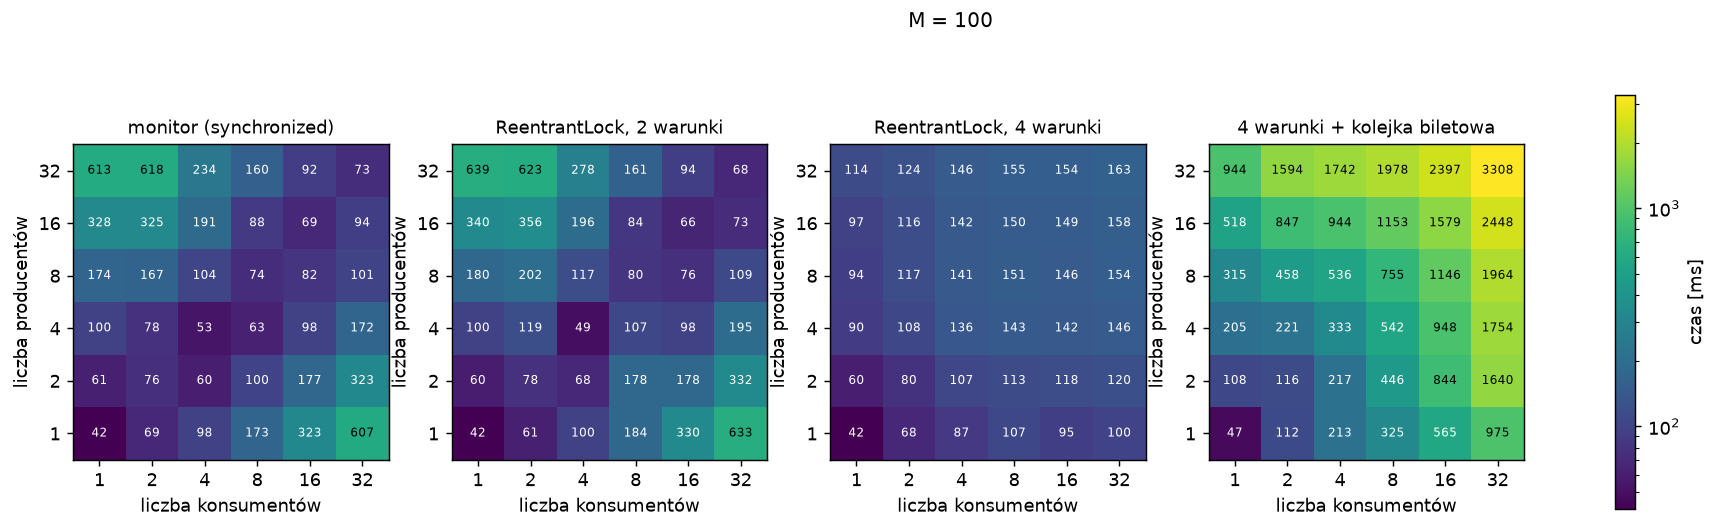
\includegraphics[width=\textwidth]{img/heatmap_100.png}
    \caption{Czas wykonania [ms] w zależności od liczby producentów i konsumentów, $M = 100$}
\end{figure}

\begin{figure}[H]
    \centering
    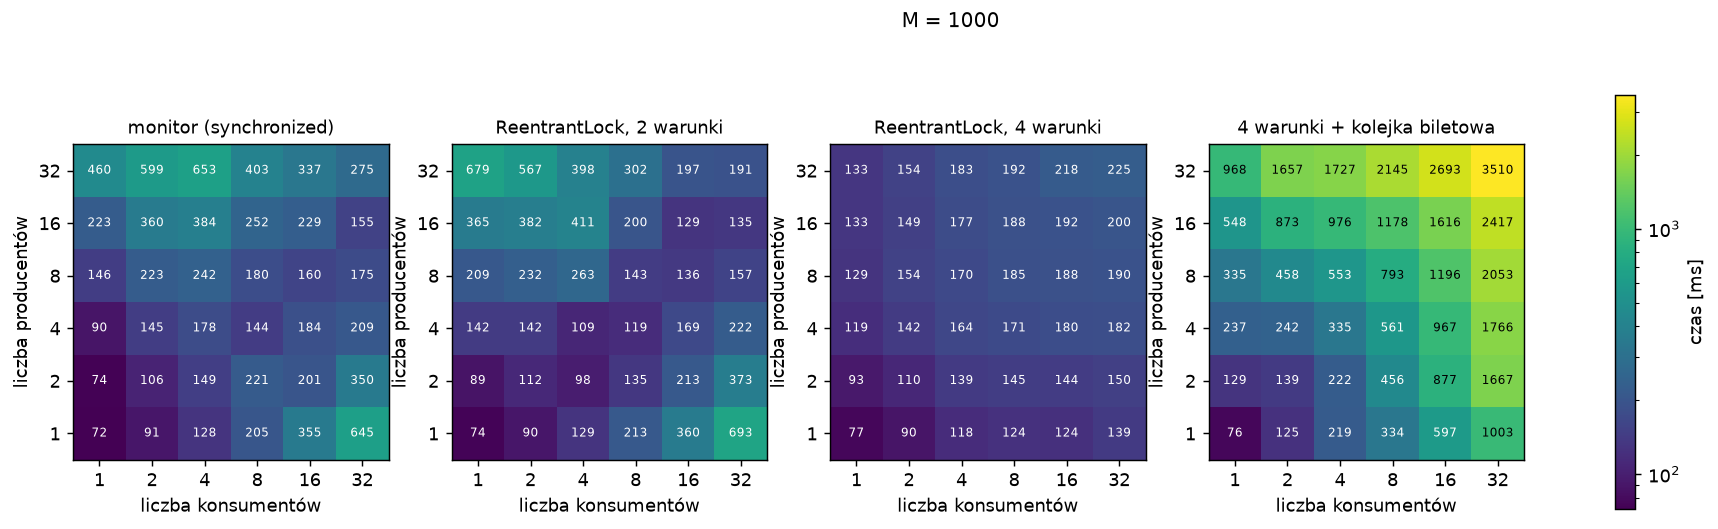
\includegraphics[width=\textwidth]{img/heatmap_1000.png}
    \caption{Czas wykonania [ms] w zależności od liczby producentów i konsumentów, $M = 1000$}
\end{figure}

\begin{figure}[H]
    \centering
    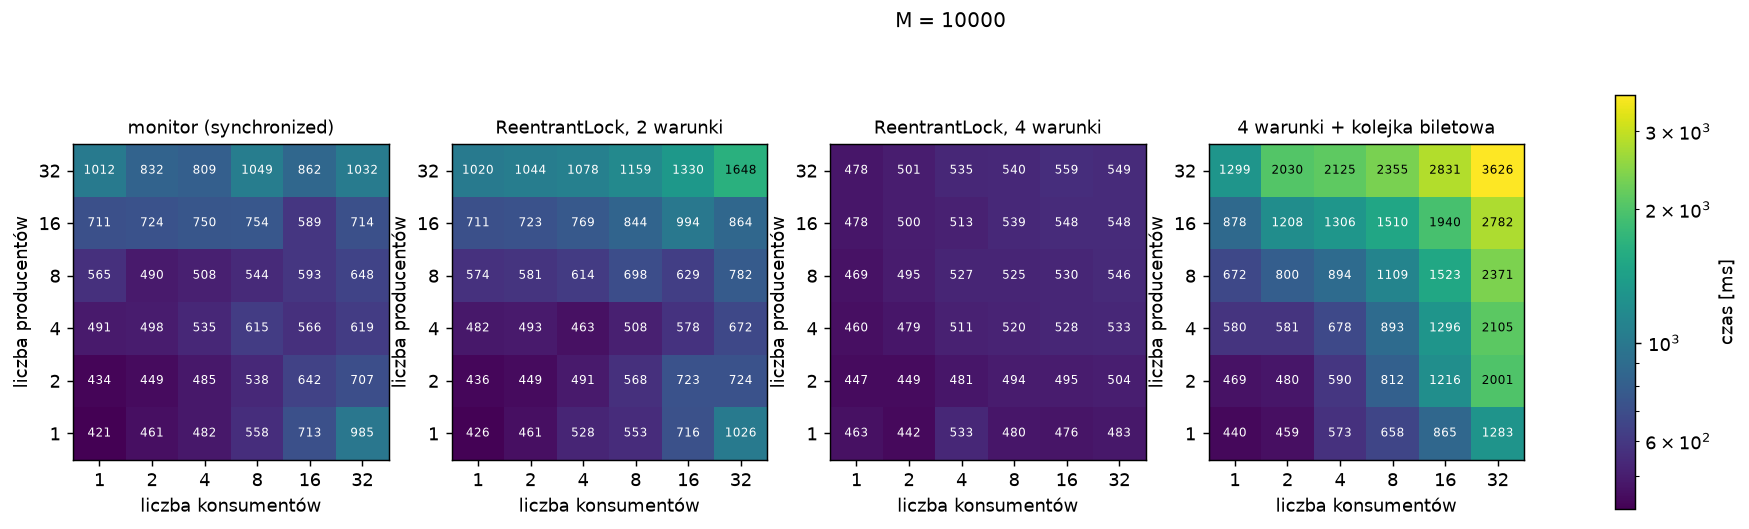
\includegraphics[width=\textwidth]{img/heatmap_10000.png}
    \caption{Czas wykonania [ms] w zależności od liczby producentów i konsumentów, $M = 10\,000$}
\end{figure}

Rozwiązania naiwne mają najgorsze czasy w rogach, czyli przy jednym producencie i 32 konsumentach
albo odwrotnie: dla $M = 1000$ jest to 460--690 ms, a przy 32 parach wątków tylko 190--275 ms.
Jedyny producent po każdym wstawieniu budzi 32 konsumentów, z których większość nie znajduje
wystarczającej liczby elementów i od razu znów czeka. W rozwiązaniu z czterema warunkami
budzi się tylko pierwszy konsument, dlatego te same konfiguracje zajmują 130--140 ms.
W kolejce biletowej czas rośnie z każdą z liczb wątków, bo dłuższa kolejka to więcej
przełączeń wątków na każdą operację.

\needspace{20\baselineskip}
\subsection{Czas oczekiwania a wielkość porcji}
\textbf{Rysunek 5} pokazuje średni czas jednego wywołania \texttt{put} i \texttt{take}
w zależności od wielkości porcji dla $M = 1000$ i 16 par wątków.

\begin{figure}[H]
    \centering
    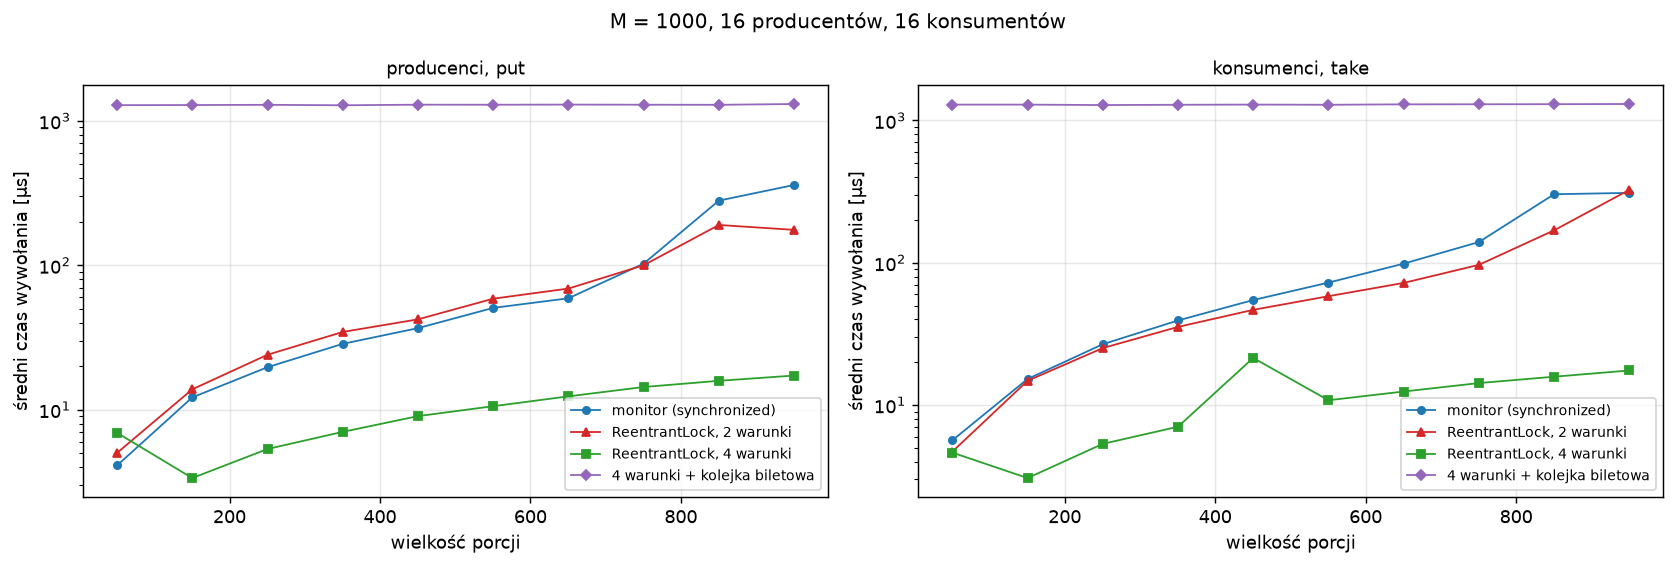
\includegraphics[width=\textwidth]{img/waits.png}
    \caption{Średni czas wywołania w zależności od wielkości porcji}
\end{figure}

W rozwiązaniach naiwnych wywołanie z porcją bliską $M$ trwa średnio 175--360 \textmu s,
a z porcją do 100 elementów 4--6 \textmu s, czyli 40--80 razy krócej. Wątki z dużymi porcjami
są wyprzedzane przez wątki z małymi, zgodnie z opisem z rozdziału \ref{sec:naive}.
W rozwiązaniu z czterema warunkami czas rośnie tylko z 7 do 17 \textmu s,
mniej więcej proporcjonalnie do liczby kopiowanych elementów.
W kolejce biletowej każde wywołanie trwa około 1,3 ms niezależnie od porcji,
bo wątek czeka, aż obsłużone zostaną wszystkie wątki przed nim w kolejce.

\needspace{20\baselineskip}
\subsection{Podział pracy między wątki}
\textbf{Rysunek 6} pokazuje indeks Jaina. Przerywana linia $\frac{1}{k}$
odpowiada sytuacji, w której całą pracę wykonuje jeden wątek.

\begin{figure}[H]
    \centering
    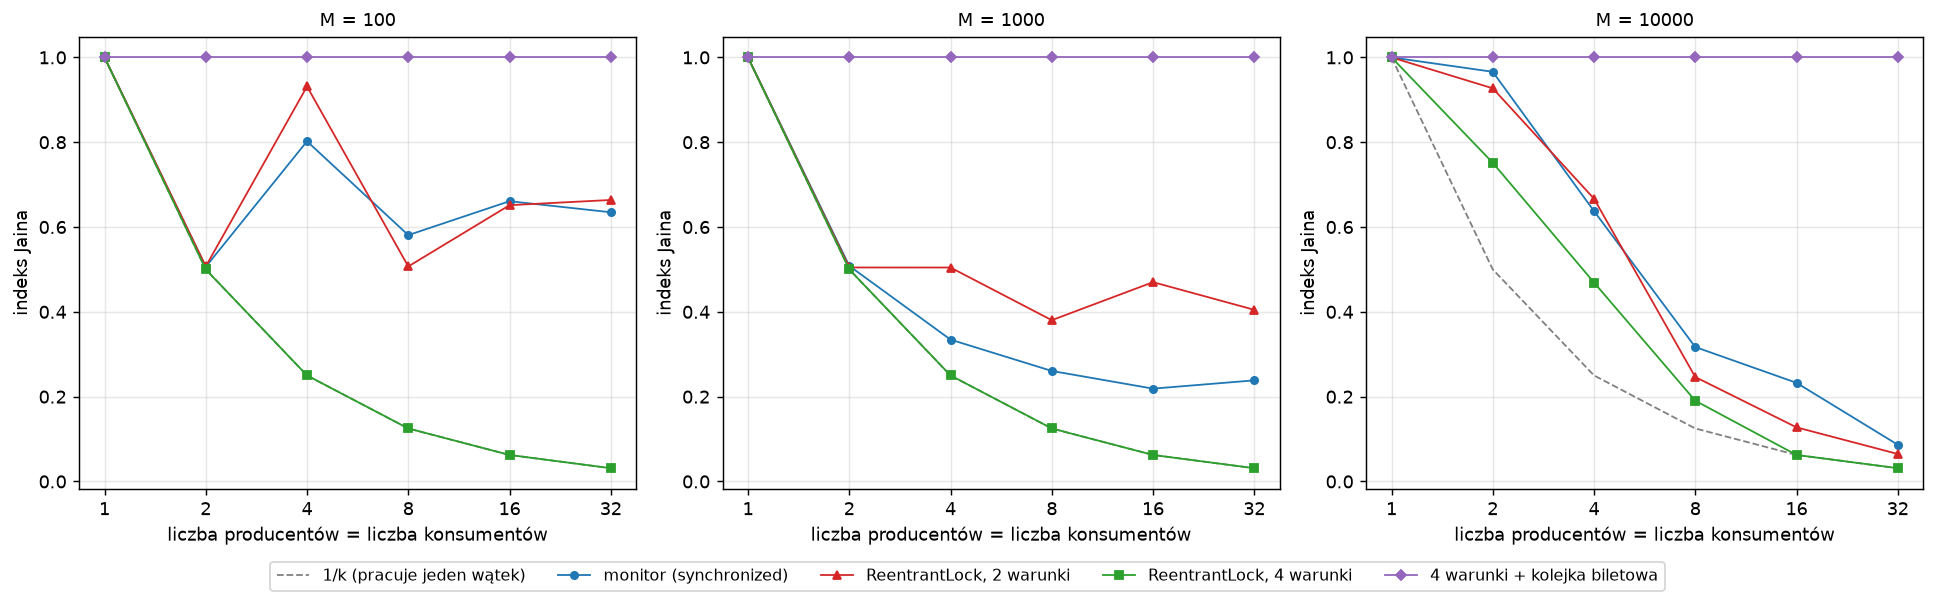
\includegraphics[width=\textwidth]{img/jain_threads.png}
    \caption{Indeks Jaina w zależności od liczby wątków dla $m = n$}
\end{figure}

Dla $M \le 1000$ rozwiązanie z czterema warunkami leży dokładnie na linii $\frac{1}{k}$:
z powodu opisanego w rozdziale \ref{sec:barging} jeden producent i jeden konsument
wykonują wszystkie operacje, a pozostałe wątki przez cały przebieg czekają.
Stąd też jego stały czas na rysunku 1: niezależnie od $k$ pracuje jedna para wątków.
Dla $M = 10\,000$ kopiowanie porcji trwa na tyle długo, że obudzony wątek czasem zdąży
zdobyć blokadę, ale od 8 par wątków indeks i tak jest bliski $\frac{1}{k}$.
Rozwiązania naiwne dzielą pracę lepiej, ale też nierówno ($J = 0{,}06$--$0{,}7$
dla 8 i więcej par wątków). Tylko kolejka biletowa daje $J = 1$ we wszystkich konfiguracjach.
Monitor \texttt{synchronized} również nie gwarantuje kolejności wejścia, więc i on pozwala
wątkowi, który właśnie wyszedł, od razu wrócić.

\section{Wnioski}
Monitor Javy i \texttt{ReentrantLock} z dwoma warunkami działają podobnie.
Dla małych porcji są najszybsze, ale wątki z dużymi porcjami czekają kilkadziesiąt razy dłużej
niż wątki z małymi, a przy nierównej liczbie producentów i konsumentów budzenie wszystkich
czekających wątków sprawia, że działają 4--5 razy dłużej niż rozwiązanie z czterema warunkami. Osobne warunki dla producentów i konsumentów
pomagają dla $M \le 1000$, ale dla $M = 10\,000$ i wielu wątków wersja z \texttt{ReentrantLock}
okazała się wolniejsza od monitora.

Rozwiązanie z czterema warunkami usuwa zależność czasu oczekiwania od wielkości porcji
i najlepiej skaluje się dla dużych porcji. Nie jest jednak sprawiedliwe względem wątków:
domyślny \texttt{ReentrantLock} pozwala wątkowi, który właśnie zwolnił blokadę, natychmiast
ją odzyskać, więc praktycznie całą pracę wykonuje jeden producent i jeden konsument.
Jego dobra wydajność wynika głównie z tego, że pozostałe wątki prawie nie biorą udziału w pracy.

Kolejka biletowa jest jedyną implementacją, w której każdy wątek wykonuje tyle samo operacji
i czeka tyle samo niezależnie od porcji. Kosztuje to jednak czas: dla 32 par wątków jest 2--7 razy wolniejsza dla $M = 10\,000$
i do 50 razy wolniejsza dla $M = 100$,
bo każda operacja wymaga przekazania pierwszego miejsca innemu, uśpionemu wątkowi.
Wybór implementacji zależy więc od tego, czy ważniejsza jest przepustowość,
czy gwarancja, że żaden wątek nie zostanie zagłodzony.

\begin{thebibliography}{9}
    \bibitem{hansen} Per Brinch Hansen: \textit{Java's Insecure Parallelism}. ACM SIGPLAN Notices, kwiecień 1999.
    \bibitem{jcu} \url{https://docs.oracle.com/en/java/javase/27/docs/api/java.base/java/util/concurrent/locks/Condition.html}
    \bibitem{jenkov} \url{https://jenkov.com/tutorials/java-util-concurrent/index.html}
\end{thebibliography}

\end{document}
